In this section outline your results. At this point, you are just stating the outcome of your analysis. You can highlight important aspects (``we observe a significantly higher value of $x$ over $y$''), but leave interpretation and opinion to the next section. This section absoultely \emph{has} to include at least two figures.


\begin{figure*}[h]
    \vskip 0.2in
    \centering
    \centerline{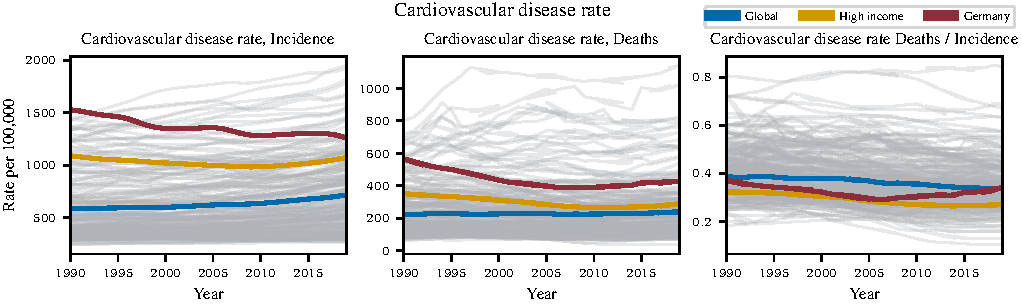
\includegraphics[]{fig/fig_cardiovascular_disease_mortality_rate.pdf}}
    \caption{Effect of the cardiovascular diseases on the world over time. From left to right: incidence rate, death rate, 
    and the ratio of death rate to incidence rate. The data is taken from the Global Burden of Disease study \citep{GBD2019}. We specifically focus on the values 
    for Germany in comparison to other high income countries and the world.}
    \label{Cardiovascular diseases over time}
\end{figure*}

% \begin{figure}[ht]
% \vskip 0.2in
% \begin{center}
% \centerline{\includegraphics[width=\columnwidth]{icml_numpapers}}
% \caption{Historical locations and number of accepted papers for International
% Machine Learning Conferences (ICML 1993 -- ICML 2008) and International
% Workshops on Machine Learning (ML 1988 -- ML 1992). At the time this figure was
% produced, the number of accepted papers for ICML 2008 was unknown and instead
% estimated.}
% \label{icml-historical}
% \end{center}
% \vskip -0.2in
% \end{figure}

% CVDs death and incidence, Permutation test
Figure \citep{GBD2019} with how it shows the real issue CVDs are in Germany compared to HIC and GLO. Talk about the permutation test. 

% plot age distribution
CVDs are way more prominent for older people (perhaps a plot for inc rate in age groups). 

% Why we focus on high income countries (already in data & methods)
% bubble plot
so comparing with all of the world countries will not give a good reasoning for life expectancy. limit ourselves to some countries with high income and high avg age (we could make a bubble plot of some sort for it) (also helps that we don't have data for all the factors for all the countries).

% analyze the factors, together or separately for healthcare and lifestyle. final plots and points
% alcohol, smoking, fat